% Graphical abstract for IEEE Access submission.
%
% Build as a standalone PDF, then convert to 300-dpi PNG or EPS:
%   pdflatex main.tex                     # produces main.pdf
%   convert -density 300 main.pdf main.png # 300 dpi PNG
%   pdftops -eps main.pdf main.eps         # EPS for IEEE Access
%
% Aspect: 16:10 (1024x640 effective, IEEE Access accepts up to 1920x1080).
%
% Layout:
%   Left  (40%) — system architecture sketch (Pillars 1-5 visible)
%   Right (60%) — 3 stacked mini-panels with headline empirical results:
%       (a) Reputation trajectory (honest vs Byzantine)
%       (b) CEP_50 vs relay depth k (bars, with 100-m NATO threshold)
%       (c) Failover timing distribution (silence-trigger vs reputation-trigger)
%
\documentclass[tikz,border=4pt]{standalone}
\usepackage{tikz}
\usetikzlibrary{arrows.meta,positioning,shapes.geometric,fit,calc,patterns}
\usepackage{xcolor}
\usepackage{amsmath}

% Colours: muted IEEE palette
\definecolor{ieeeblue}{HTML}{0072BC}
\definecolor{ieeered}{HTML}{D7263D}
\definecolor{ieeegreen}{HTML}{2E933C}
\definecolor{ieeeamber}{HTML}{F2A900}
\definecolor{ieeegrey}{HTML}{6E6E6E}

\begin{document}
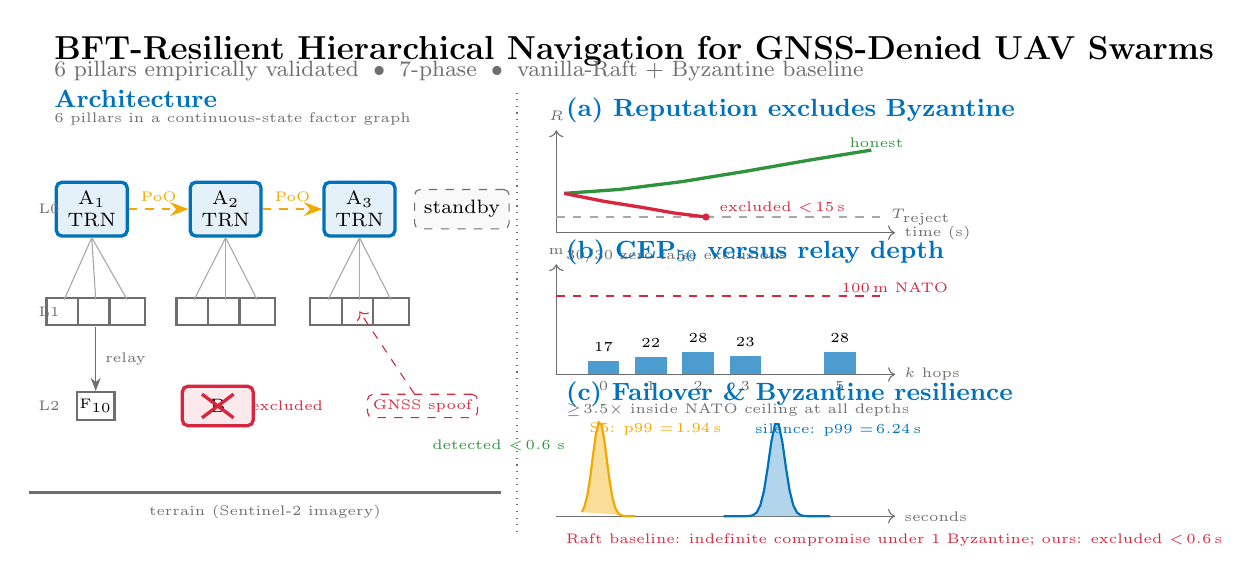
\begin{tikzpicture}[
    anchorbox/.style={draw=ieeeblue, very thick, rectangle, rounded corners=2pt,
                      minimum width=0.9cm, minimum height=0.5cm, font=\scriptsize,
                      align=center, fill=ieeeblue!10},
    follower/.style ={draw=ieeegrey, thick, rectangle, minimum width=0.45cm,
                      minimum height=0.35cm, font=\tiny, inner sep=1pt, align=center,
                      fill=white},
    standby/.style  ={draw=ieeegrey, dashed, rectangle, rounded corners=2pt,
                      minimum width=0.9cm, minimum height=0.5cm, font=\scriptsize,
                      align=center, fill=gray!5},
    byzantine/.style={draw=ieeered, very thick, rectangle, rounded corners=2pt,
                      minimum width=0.9cm, minimum height=0.5cm, font=\scriptsize,
                      align=center, fill=ieeered!10},
    panel/.style    ={draw=ieeegrey, thick, rectangle, rounded corners=3pt,
                      inner sep=4pt, fill=white},
]

% =========================================================================
% LEFT PANEL — system architecture sketch
% =========================================================================
\begin{scope}[shift={(0,0)}]
    % Section title
    \node[anchor=west, font=\small\bfseries, ieeeblue]
        at (-0.3, 5.1) {Architecture};
    \node[anchor=west, font=\tiny, ieeegrey]
        at (-0.3, 4.85) {6 pillars in a continuous-state factor graph};

    % Active anchors (Pillar 2: hierarchical)
    \node[anchorbox] (A1) at (0.3, 3.7) {A$_1$\\TRN};
    \node[anchorbox] (A2) at (2.0, 3.7) {A$_2$\\TRN};
    \node[anchorbox] (A3) at (3.7, 3.7) {A$_3$\\TRN};
    \node[standby]   (S1) at (5.0, 3.7) {standby};

    % PoO mutual verification (Pillar 1)
    \draw[dashed, -{Stealth}, thick, ieeeamber]
        (A1) -- node[above, font=\tiny, ieeeamber, yshift=-1pt] {PoO} (A2);
    \draw[dashed, -{Stealth}, thick, ieeeamber]
        (A2) -- node[above, font=\tiny, ieeeamber, yshift=-1pt] {PoO} (A3);

    % Followers under each anchor (Pillar 3: relay)
    \foreach \x/\n in {-0.05/F$_1$, 0.35/F$_2$, 0.75/F$_3$} {
        \node[follower] (\n) at (\x, 2.4) {};
        \draw[-, ieeegrey!60] (A1.south) -- (\x, 2.55);
    }
    \foreach \x/\n in {1.6/F$_4$, 2.0/F$_5$, 2.4/F$_6$} {
        \node[follower] at (\x, 2.4) {};
        \draw[-, ieeegrey!60] (A2.south) -- (\x, 2.55);
    }
    \foreach \x/\n in {3.3/F$_7$, 3.7/F$_8$, 4.1/F$_9$} {
        \node[follower] at (\x, 2.4) {};
        \draw[-, ieeegrey!60] (A3.south) -- (\x, 2.55);
    }

    % Level 2 (relayed)
    \node[follower] (FR) at (0.35, 1.2) {F$_{10}$};
    \draw[-{Stealth}, ieeegrey] (0.35, 2.2) -- (FR)
        node[midway, right, font=\tiny] {relay};

    % Byzantine attacker (excluded; Pillar 1+3)
    \node[byzantine] (BX) at (1.9, 1.2) {B};
    \draw[-, ieeered, very thick] (1.7, 1.05) -- (2.1, 1.35);
    \draw[-, ieeered, very thick] (1.7, 1.35) -- (2.1, 1.05);
    \node[font=\tiny, ieeered, anchor=west] at (2.2, 1.2) {excluded};

    % GNSS spoofer (Pillar 5)
    \node[font=\tiny, ieeered, draw=ieeered, dashed,
          rounded corners=2pt, inner sep=2pt] (SP) at (4.5, 1.2)
        {GNSS spoof};
    \draw[->, ieeered, dashed] (SP) -- (3.7, 2.4);
    \node[font=\tiny, ieeegreen, anchor=west] at (4.5, 0.7)
        {detected $<\!0.6$ s};

    % Terrain baseline
    \draw[thick, ieeegrey] (-0.5, 0.1) -- (5.5, 0.1);
    \node[font=\tiny, ieeegrey] at (2.5, -0.15) {terrain (Sentinel-2 imagery)};

    % Level labels
    \node[font=\tiny, ieeegrey, anchor=west] at (-0.5, 3.7) {L0};
    \node[font=\tiny, ieeegrey, anchor=west] at (-0.5, 2.4) {L1};
    \node[font=\tiny, ieeegrey, anchor=west] at (-0.5, 1.2) {L2};

    % Boundary
    \draw[ieeegrey, dotted] (5.7, -0.4) -- (5.7, 5.2);
\end{scope}

% =========================================================================
% RIGHT PANEL (a) — Reputation trajectory
% =========================================================================
\begin{scope}[shift={(6.2,3.4)}]
    \node[anchor=west, font=\small\bfseries, ieeeblue]
        at (0, 1.55) {(a) Reputation excludes Byzantine};
    % Axes
    \draw[->, ieeegrey] (0, 0) -- (4.3, 0) node[right, font=\tiny] {time (s)};
    \draw[->, ieeegrey] (0, 0) -- (0, 1.3) node[above, font=\tiny] {$R$};
    % Threshold
    \draw[dashed, ieeegrey!60] (0, 0.2) -- (4.2, 0.2);
    \node[font=\tiny, ieeegrey] at (4.2, 0.2) [right, xshift=-2pt] {$T_\text{reject}$};
    % Honest trajectory (rising)
    \draw[very thick, ieeegreen] plot coordinates
        {(0.1, 0.5) (0.8, 0.55) (1.6, 0.65) (2.4, 0.78) (3.2, 0.92)
         (4.0, 1.05)};
    \node[ieeegreen, font=\tiny, anchor=west] at (3.6, 1.15) {honest};
    % Byzantine trajectory (falling)
    \draw[very thick, ieeered] plot coordinates
        {(0.1, 0.5) (0.6, 0.4) (1.1, 0.32) (1.5, 0.25) (1.9, 0.2)};
    \fill[ieeered] (1.9, 0.2) circle (1.3pt);
    \node[ieeered, font=\tiny, anchor=west] at (1.95, 0.32) {excluded $<\!15$\,s};
    % Annotation
    \node[font=\tiny, ieeegrey, anchor=west] at (0.0, -0.3)
        {30/30 zero false exclusions};
\end{scope}

% =========================================================================
% RIGHT PANEL (b) — CEP_50 vs relay depth (bar chart)
% =========================================================================
\begin{scope}[shift={(6.2,1.6)}]
    \node[anchor=west, font=\small\bfseries, ieeeblue]
        at (0, 1.55) {(b) CEP$_{50}$ versus relay depth};
    % Axes
    \draw[->, ieeegrey] (0, 0) -- (4.3, 0) node[right, font=\tiny] {$k$ hops};
    \draw[->, ieeegrey] (0, 0) -- (0, 1.4) node[above, font=\tiny] {m};
    % 100-m NATO threshold (scaled: 100 m -> y=1.0)
    \draw[dashed, ieeered, thick] (0, 1.0) -- (4.2, 1.0);
    \node[font=\tiny, ieeered, anchor=west] at (3.5, 1.1) {100\,m NATO};
    % Bars: k=0 17m, k=1 22m, k=2 28m, k=3 23m, k=5 28m → /100 = heights
    \foreach \x/\h/\lab in {0.4/0.17/17, 1.0/0.22/22, 1.6/0.28/28,
                            2.2/0.23/23, 3.4/0.28/28} {
        \fill[ieeeblue!70] (\x, 0) rectangle ({\x+0.4}, \h);
        \node[font=\tiny, anchor=south] at ({\x+0.2}, \h) {\lab};
    }
    \foreach \x/\k in {0.6/0, 1.2/1, 1.8/2, 2.4/3, 3.6/5} {
        \node[font=\tiny, ieeegrey] at (\x, -0.15) {\k};
    }
    % Margin annotation
    \node[font=\tiny, ieeegrey, anchor=west] at (0, -0.45)
        {$\geq\!3.5\times$ inside NATO ceiling at all depths};
\end{scope}

% =========================================================================
% RIGHT PANEL (c) — Failover timing
% =========================================================================
\begin{scope}[shift={(6.2,-0.2)}]
    \node[anchor=west, font=\small\bfseries, ieeeblue]
        at (0, 1.55) {(c) Failover \& Byzantine resilience};
    % Axes
    \draw[->, ieeegrey] (0, 0) -- (4.3, 0) node[right, font=\tiny] {seconds};
    % Silence-triggered (S1-S3) — narrow bell at 6s
    \draw[fill=ieeeblue!30, draw=ieeeblue, thick] plot[domain=4.5:7.5, samples=30]
        ({\x*0.45 + 0.1}, {1.2*exp(-((\x-6)^2)/0.10)});
    \node[font=\tiny, ieeeblue, anchor=west] at (2.4, 1.1)
        {silence: p99 $=\!6.24$\,s};
    % Reputation-triggered (S5) — narrow bell at 1s
    \draw[fill=ieeeamber!40, draw=ieeeamber, thick] plot[domain=0.5:2.0, samples=20]
        ({\x*0.45 + 0.1}, {1.2*exp(-((\x-1)^2)/0.08)});
    \node[font=\tiny, ieeeamber, anchor=west] at (0.3, 1.1)
        {S5: p99 $=\!1.94$\,s};
    % BFT-vs-CFT gap annotation
    \node[font=\tiny, ieeered, anchor=west] at (0.0, -0.3)
        {Raft baseline: indefinite compromise under 1 Byzantine; ours: excluded $<\!0.6$\,s};
\end{scope}

% =========================================================================
% Title across top
% =========================================================================
\node[anchor=west, font=\large\bfseries] at (-0.3, 5.7)
    {BFT-Resilient Hierarchical Navigation for GNSS-Denied UAV Swarms};
\node[anchor=west, font=\footnotesize, ieeegrey] at (-0.3, 5.45)
    {6 pillars empirically validated $\;\bullet\;$ 7-phase $\;\bullet\;$ vanilla-Raft + Byzantine baseline};

\end{tikzpicture}
\end{document}
